%%=============================================================================
%% Methodologie
%%=============================================================================

\chapter{\IfLanguageName{dutch}{Methodologie}{Methodology}}%
\label{ch:methodologie}

%% TODO: In dit hoofstuk geef je een korte toelichting over hoe je te werk bent
%% gegaan. Verdeel je onderzoek in grote fasen, en licht in elke fase toe wat
%% de doelstelling was, welke deliverables daar uit gekomen zijn, en welke
%% onderzoeksmethoden je daarbij toegepast hebt. Verantwoord waarom je
%% op deze manier te werk gegaan bent.
%% 
%% Voorbeelden van zulke fasen zijn: literatuurstudie, opstellen van een
%% requirements-analyse, opstellen long-list (bij vergelijkende studie),
%% selectie van geschikte tools (bij vergelijkende studie, "short-list"),
%% opzetten testopstelling/PoC, uitvoeren testen en verzamelen
%% van resultaten, analyse van resultaten, ...
%%
%% !!!!! LET OP !!!!!
%%
%% Het is uitdrukkelijk NIET de bedoeling dat je het grootste deel van de corpus
%% van je bachelorproef in dit hoofstuk verwerkt! Dit hoofdstuk is eerder een
%% kort overzicht van je plan van aanpak.
%%
%% Maak voor elke fase (behalve het literatuuronderzoek) een NIEUW HOOFDSTUK aan
%% en geef het een gepaste titel.

In de initiële fase van dit onderzoek, de literatuurstudie, werd de focus gelegd op het verzamelen van bestaande kennis 
en onderzoek op het gebied van webapplicatiebeveiliging, pentesting-tools en frameworks, met een specifieke nadruk op 
de doelomgevingen WordPress en Laravel. Deze fase was van cruciaal 
belang om een stevige basis te leggen voor dit onderzoek en om de context en achtergrond van het onderwerp volledig te 
begrijpen.

Om dit te bereiken, werden verschillende bronnen geraadpleegd, waaronder wetenschappelijke artikelen, boeken  
en rapporten van bekende instellingen en experts op het gebied van cybersecurity. 
Ook werden zoekopdrachten uitgevoerd in diverse academische databases, zoals PubMed, research gate en 
Google Scholar om relevante en onderbouwde literatuur op te nemen in de studie. Deze literatuur is grondig geanalyseerd en 
samengevat, waarbij de nadruk werd gelegd op recente ontwikkelingen, trends en mogelijke tekortkomingen in de bestaande markt.
Ook werd in dit deel het globale aspect van cybersecutiy onder de loep genomen waardoor er een zeer duidelijk begrip 
is van de noden en hoe hierop een antwoord werd gegeven.

\section{\IfLanguageName{dutch}{Requirements Analyse}{Requirements analysis}}
De requirements analyse vormt een cruciaal luik en beschrijft de methoden en technieken die werden toegepast 
voor het uitvoeren van penetratietests. In deze studie werden deze toegepast op twee 
verschillende webomgevingen met name een WordPress CMS-framework en een Laravel-applicatie. Het doel van deze tests is om kwetsbaarheden te identificeren, te 
analyseren en de effectiviteit van de beveiligingsmaatregelen en aanvalstrategieën in de beide omgevingen te vergelijken.
Deze twee doelomgevingen zijn geselecteerd op basis van hun populariteit en relevantie voor kleine tot middelgrote bedrijven 
zoals webdevelopment firma Sinergio, die de partner en co-promotor is in dit onderzoek.

Bij de start van deze studie werden eerst de nodige keuzes en methodieken verklaard en verantwoord. De manier waarop deze keuzes zijn gemaakt, werd eveneens 
besproken, zodat dit in een latere fase van het onderzoek kan worden uitgevoerd.

Dit onderzoek is opgesplitst in twee delen waarbij in de initiële fase gefocust werd op de keuze van de meest passende pentesting tool 
aan de hand van vooropgestelde criteria. Hierop gebaseerd werden drie pentestingtools gekozen die op hun beurt werden vergeleken met elkaar 
zodat er in de tweede fase van het onderzoek op een solide basis kan worden verder gebouwd. In deze fase zal met één geselecteerde 
tool dertien pentests worden afgenomen op de omgevingen waarbij er binnen de testen op een wordpress CMS systeem nog onderscheid zal worden gemaakt 
tussen een versie met en een versie zonder beveiligingsplugin.

\subsection{\IfLanguageName{dutch}{Keuze van pentesttools}{choice of pentesttools}}
Voor dit onderzoek is het van 
belang dat tools werden gebruikt met vergelijkbare functionaliteiten, maar met verschillende intrinsieke accenten om te bepalen welke 
tool het meest geschikt is binnen de hiervoor besproken scenario's. In het kader van deze proef is het belangrijk dat er voldoende onderscheid is tussen de tools 
die werden vergeleken, zodat in de conclusie duidelijk wordt welke pentesttool het meest geschikt en toepasselijk is in deze context. 
Pentesting-tools zoals Nmap of Wireshark zijn bijvoorbeeld vooral gericht op het testen van netwerken en  zijn daarom minder van toepassing. Er werd 
gediversifieerd door te selecteren in de open source toepassingen versus propriety software, waarbij in dit laatste geval de gratis versie werd 
verkozen. 

Aangezien de pentesttool bij voorkeur kost efficiënt dient te zijn in dit onderzoek, is het voor de hand liggend om een open-source tool te gebruiken. Precies daarom 
is dit een factor waarom de vergelijking gemaakt wordt tussen een gratis versie van een pentesting tool en een (uiteraard gratis) open-source tool. 
Tevens werd één tool geselecteerd waarbij de pentesting-capaciteiten verder gaan dan alleen het testen van webapplicaties, met een 
uitgebreider scala aan mogelijkheden zoals het testen van netwerken of mobiele applicaties. Op die manier werd duidelijk dat dit 
de doeltreffendheid van de pentesten bevordert.

Op basis van de bovenstaande criteria werden de volgende pentest toepassingen weerhouden:
\begin{itemize}
    \item Metasploit: open-source software met en een uitgebreider scala aan functionaliteiten die niet enkel beperken tot webapplicatie testings.
    \item Burp suite: geen open-source software die bovendien alleen ingezet wordt voor het testen van webapplicaties.
    \item OWASP ZAP: open-source software die eveneens enkel gebruikt wordt voor het testen van webapplicaties.
\end{itemize}

De daaropvolgende keuze tussen de drie weerhouden pentesttools is gebaseerd op vooraf vastgestelde globale criteria, waarbij de nadruk ligt op welke tool het meest 
geschikt is voor het testen van de opgezette omgevingen (wordpress CMS en Laravel applicatie). Deze criteria omvatten:
\begin{itemize}
    \item De omvang van het scala aan capaciteiten en functionaliteiten voor het testen van webapplicaties.
    \item Resourcegebruik met name CPU-, geheugen- en netwerkgebruik.
    \item Ondersteuning door de community, door de gemiddelde antwoordtijd van reacties van 20 laatste openstaande issues te vergelijken.
\end{itemize}

Bij de selectie van de te weerhouden pentesting-tool voor dit onderzoek werd eerst een eigen analyse gemaakt op basis van deze bovenstaande criteria. 
Nadien werd een analyse gemaakt van gebruikerservaringen van derden. Dit gebeurt aan de hand van beoordelingen en recensies van 
verschillende gebruikers, waarbij de pro's en contra's die de reviewers vermelden in overweging werd genomen. 

Op g2.com en peerspot.com bestaat de 
mogelijkheid om reviews van deze tools naast elkaar te leggen. Beide zijn bewezen betrouwbare platformen voor het beoordelen 
van pentesttools aan de hand van gebruiker-bepaalde pro's en contra's volgens trustradius. 

Deze vergelijking door derden is belangrijk in deze studie, aangezien het niet haalbaar is om een volledig framework 
autonoom te evalueren zonder rekening te houden met de mening van anderen met een uitgebreidere expertise of ervaring. Daarom 
is het van groot belang om ook de conclusies van externe partijen mee te nemen, die mogelijk andere 
aspecten hebben waargenomen. Op basis van deze laatste analyse werd geconcludeerd welke pentesting-tool het meest 
geschikt is voor gebruik in deze context.

\subsection{\IfLanguageName{dutch}{Aanpak van web omgevingen}{Use of web enviroments}}
Voorafgaand aan de uitvoering van de penetratietests werd in samenspraak Sinergio, met de partner van deze bachelorproef, drie 
webapplicaties opgezet waarop de testen werden uitgevoerd. Om de business impact minimaal te houden werd hiertoe een 
aparte test-server opgezet. Alle tests werden overigens uitgevoerd in overeenstemming met de ethische 
richtlijnen voor cybersecurityonderzoek, waarbij de integriteit van de geteste systemen vooropstaat. De te testen 
webapplicaties zijn de onderstaande en bereikbaar via de bijhorende link:

\begin{itemize}
    \item WordPress-applicatie met beveiligingsplugins: Deze applicatie maakt gebruik van WordPress versie 6.5.5 en wordt 
    beschermd door de Wordfence-plugin. Bijkomende plugins die op de omgeving zijn geïnstalleerd, zijn Elementor 
    (gebruikt als page builder en theme builder voor WordPress) en Forminator (aanmaken van eenvoudige formulierenwat noodzakelijk is voor de testen).  
    De website is toegankelijk via: \url{https://testlevi.abako.be/}
    \item WordPress-applicatie zonder beveiligingsplugins: Deze website heeft gelijkaardige instellingen als de bovenstaande, 
    met als enige verschil het ontbreken van de Wordfence-plugin: \url{https://testlevi2.abako.be/}
    \item Laravel applicatie: De web omgeving maakt gebruik van Laravel framework versie 10.10 \url{https://testlevi3.abako.be/}
\end{itemize}

Binnen het onderzoek werd voornamelijk geanalyseerd welke omgeving het meest robuust is tegen verschillende uitgevoerde pentestaanvallen. 
Het is daarom belangrijk om de juiste kwetsbaarheden te testen, zodat een correcte en volledige conclusie kan worden 
getrokken. De geselecteerde kwetsbaarheden zijn gebaseerd op de OWASP Top 10, een lijst van de tien belangrijkste 
kwetsbaarheden binnen de cybersecuritywereld. Niet alle kwetsbaarheden uit deze lijst kunnen echter worden getest met de 
gekozen pentesting-tool, aangezien deze op serverniveau te testen zijn. Dit heeft geleid tot de volgende uitgevoerde pentests:

\begin{itemize}
    \item SQL injection aanval
    \item Brute force aanval
    \item Sensitive data exposure
    \item Security misconfiguration
    \item Cross site scripting
    \item Insecure deserialization
    \item Insufficient logging \& monitoring 
\end{itemize}

Alle resultaten van de tests werden verzameld en gedocumenteerd. De data werd geanalyseerd 
om de ernst en de impact van elke gevonden kwetsbaarheid te bepalen. Deze analyse helpt niet alleen bij 
het identificeren van de zwakke punten binnen elke webomgeving, maar ook bij het vergelijken van de 
veiligheid tussen de verschillende systemen.

\section{\IfLanguageName{dutch}{Keuze van Penetratietesttools}{Selection of pentesttools}}
In het kader van dit onderzoek naar de beveiliging van de drie verschillende webomgevingen is de keuze van 
de juiste penetratietesttools cruciaal. De geselecteerde tools zijn 
Metasploit, Burp Suite en OWASP ZAP, waarbij hierna wordt toegelicht wat hen bijzonder geschikt maken voor dit onderzoek.
\begin{figure}
    \centering
    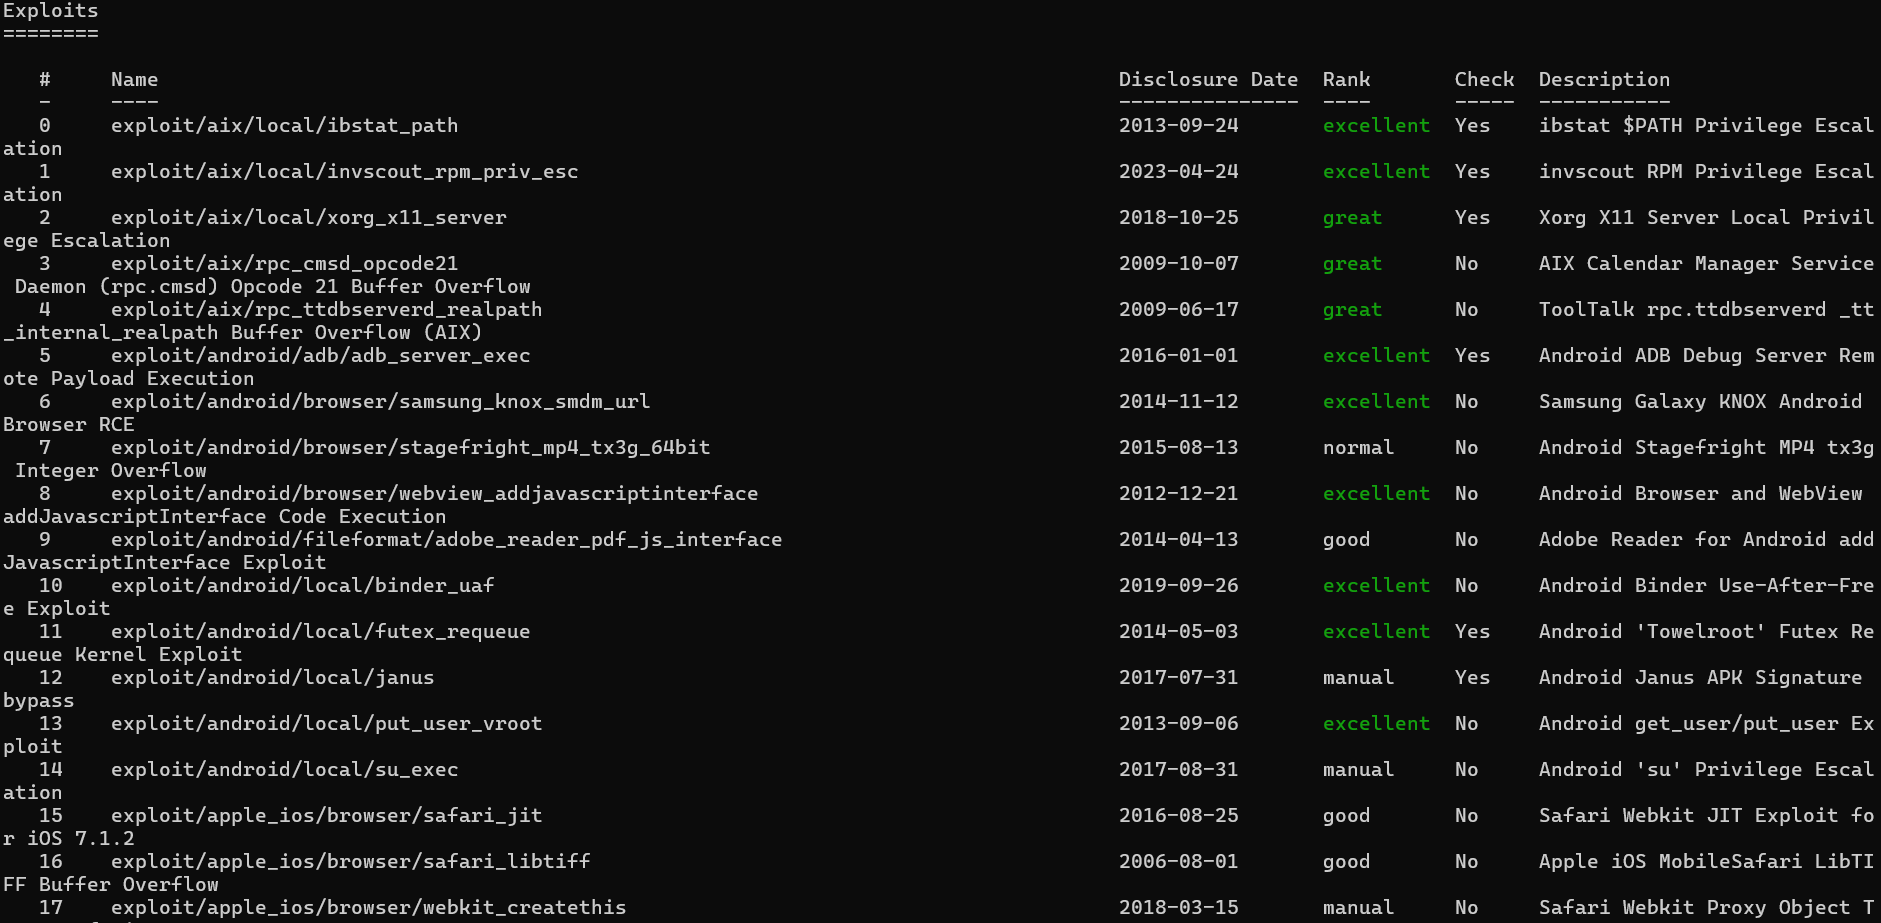
\includegraphics[height=0.3\textheight]{metasploit_exploit_db.png}
    \caption[exploitation database van metasploit]{exploitation database van metasploit}
    \label{fig:exploitatie_db}
\end{figure}
\subsection{\IfLanguageName{dutch}{Metasploit}{Metasploit}}
Metasploit is een van de meest uitgebreide security frameworks voor het uitvoeren van penetratietests en staat bekend om 
zijn robuuste exploit-database, waarvan een deel te zien is op de bovenstaande foto \ref{fig:exploitatie_db} en zoals vermeld is in het hoofdstuk \nameref{sec:Pentesting tools} van de 
literatuurstudie. Het framework biedt het vermogen om specifieke exploits te gebruiken die zijn afgestemd op gedetecteerde 
kwetsbaarheden. Metasploit biedt bovendien geautomatiseerde exploitatie-technieken, die essentieel zijn voor het identificeren 
van beveiligingsrisico's in geavanceerde frameworks zoals Laravel. 

Daarnaast ondersteunt Metasploit de ontwikkeling van 
aangepaste exploits en biedt het integratie met andere tools zoals Nmap en Wireshark, wat de veelzijdigheid en het 
gebruiksgemak verder vergroot. 

Een andere belangrijke functie is de mogelijkheid om uitgebreide rapportages te genereren, 
wat cruciaal is voor het documenteren van bevindingen en het communiceren van resultaten naar Sinergio en stakeholders. Dankzij de grote 
community en voortdurende updates blijft Metasploit relevant en actueel, wat het tot een essentieel hulpmiddel maakt in het 
testen van webapplicaties.

\subsection{\IfLanguageName{dutch}{Burp Suite}{Burp Suite}}
Burp Suite is een platform voor het testen van de beveiliging van webapplicaties en is bijzonder effectief voor 
het analyseren van HTTP-verkeer en het uitvoeren van geavanceerde webaanvallen. Zoals aangehaald in het hoofdstuk \nameref{sec:Pentesting tools} 
van de literatuurstudie, biedt Burp Suite uitgebreide functionaliteiten die essentieel zijn voor een grondige beveiligingsanalyse 
van webomgevingen. Dankzij het vermogen om verzoeken te onderscheppen, te manipuleren en opnieuw te versturen, kunnen 
testers nauwkeurig de robuustheid beoordelen van beveiligingsmaatregelen zoals firewalls en inbraakdetectiesystemen die via 
plugins of op serverniveau worden geïmplementeerd. 

De Community Edition van Burp Suite biedt basisfunctionaliteiten, zoals de proxy en repeater, 
waarmee handmatige testactiviteiten kunnen worden uitgevoerd. Met de Proxy kunnen testers bijvoorbeeld HTTP(S)-verkeer 
onderscheppen en manipuleren voordat het de server bereikt, wat hen in staat stelt om kwetsbaarheden zoals injection flaws 
te ontdekken door bijvoorbeeld SQL-commando's in te voegen in velden die normaal gesproken niet kwetsbaar lijken. Testers 
kunnen ook cookies en headers inspecteren en aanpassen, wat helpt bij het ontdekken van session hijacking of cookie 
manipulation kwetsbaarheden.

De Repeater stelt testers in staat om specifieke HTTP-verzoeken meerdere keren handmatig te versturen, waarbij elke keer 
kleine wijzigingen kunnen worden aangebracht. Dit is bijzonder nuttig voor het testen van de robuustheid van 
input-validatiesystemen en het verfijnen van aanvallen zoals Cross-Site Scripting (XSS) of Brute force attack. Door 
herhaaldelijk verzoeken met variaties te versturen, kunnen testers de reacties van de server analyseren en mogelijke 
kwetsbaarheden identificeren.

Hoewel de Community Edition beperkingen heeft ten opzichte van de 
commerciële edities, is het nog steeds een krachtig hulpmiddel voor basisbeveiligingsanalyses en een waardevolle aanvulling 
voor beginnende testers. De scanner in de betalende Enterprise Edition van Burp Suite kan automatisch een breed scala aan kwetsbaarheden 
identificeren, wat tijd bespaart tijdens de testfase en zorgt voor een grondige evaluatie van de beveiligingsstatus.

\subsection{\IfLanguageName{dutch}{OWASP ZAP}{OWASP ZAP}}
OWASP ZAP (Zed Attack Proxy) is een open-source tool die zich richt op het automatisch detecteren van beveiligingsfouten in 
webapplicaties tijdens het ontwikkelings- en testproces. Met ZAP's geïntegreerde scanner en intercepting proxy kunnen 
kwetsbaarheden zoals Cross-Site Scripting (XSS) en SQL-injectie eenvoudig worden opgespoord. ZAP biedt 
daarnaast dynamische analyse van applicaties in real-time, waardoor beveiligingsproblemen onmiddellijk kunnen worden geïdentificeerd 
en aangepakt.

De tool is bijzonder nuttig voor zowel ontwikkelaars als beveiligingsexperts, doordat het hen in staat stelt 
om continue beveiligingstesten uit te voeren tijdens de gehele levenscyclus van een webapplicatie. Dit zorgt ervoor dat 
OWASP ZAP een zeer aantrekkelijke keuze is voor het ontwikkel team van Sinergio.
\begin{figure}
    \centering
    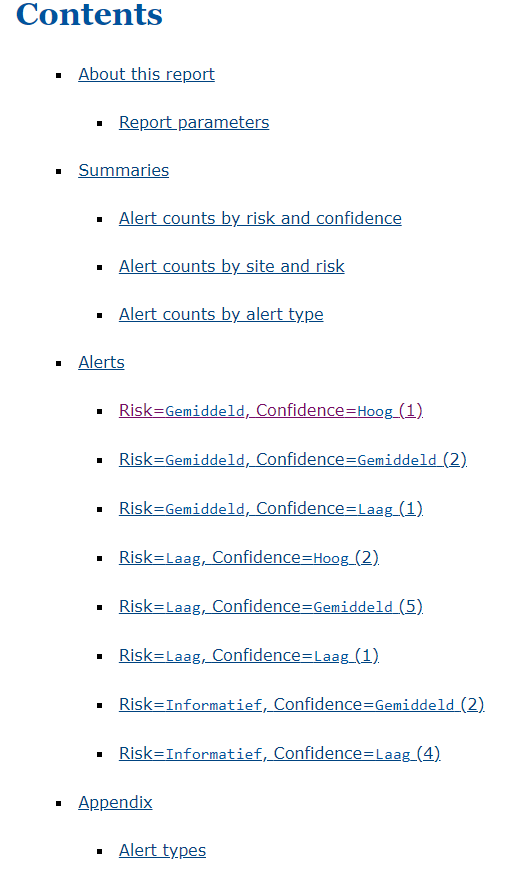
\includegraphics[height=0.3\textheight]{ZAP_report.png}
    \caption[Voorbeeld rapportage van vanuit OWASP ZAP]{Voorbeeld rapportage van vanuit OWASP ZAP}
    \label{fig:zap_report}
\end{figure}
ZAP is bovendien sterk uitbreidbaar dankzij zijn robuuste add-on marktplaats, waarmee gebruikers extra functionaliteiten 
kunnen toevoegen voor specifieke beveiligingstests. 

Een ander belangrijk aspect is de actieve en ondersteunende community 
rond OWASP ZAP, die regelmatig updates en nieuwe functies uitbrengt, waardoor de tool up-to-date blijft met de nieuwste 
beveiligingstrends en bedreigingen. ZAP biedt ook geautomatiseerde rapportagefuncties die gedetailleerde inzichten geven 
in de gevonden kwetsbaarheden zoals op bovenstaande foto \ref{fig:zap_report}. Dit is essentieel voor het documenteren van testresultaten en het verbeteren van de beveiliging 
van webapplicaties. 

\section{\IfLanguageName{dutch}{ Verkozen webomgevingen }{ chosen webenviroments }}
Voor de tests wordt gebruikgemaakt van het WordPress CMS-framework en Laravel. Deze frameworks zijn gekozen vanwege hun 
populariteit bij KMO's en middelgrote bedrijven zoals Sinergio. Binnen Sinergio wordt WordPress voornamelijk verkozen vanwege 
zijn grote populariteit, gebruiksvriendelijkheid en het feit dat het open-source is. Het brede scala aan plugins en de 
blijvende ondersteuning vanuit de community hebben Sinergio mede overtuigd om te kiezen voor dit platform. 


Laravel daarentegen is door Sinergio gekozen vanwege de eenvoud bij upgrades. Het is bijvoorbeeld mogelijk om ontwikkelde webtoepassingen 
te upgraden naar een nieuwere versie van Laravel zonder dat gegevens verloren gaan. De kennis van Laravel was 
reeds aanwezig binnen Sinergio waardoor de keuze voor dit framework snel gemaakt was. Ook de ingebouwde beveiligingsmaatregelen 
van Laravel, zoals de Eloquent ORM (hier word later op terug gekomen), hebben bijgedragen aan de keuze voor dit framework.

\subsection{\IfLanguageName{dutch}{Sinergio}{Sinergio}}
Sinergio is een bedrijf met een passie voor het ontwerpen van websites of webshops en blinkt 
uit in het maken van krachtige cloud-applicaties. Met een team van 6 medewerkers is Sinergio een kleine KMO op de markt 
die zich voornamelijk richt op het ontwikkelen van webapplicaties en websites voor KMO's en grote bedrijven. De focus 
van Sinergio ligt op het ontwikkelen van kwalitatieve maatwerkoplossingen die aansluiten bij de behoeften van hun klanten.

\begin{figure}
    \centering
    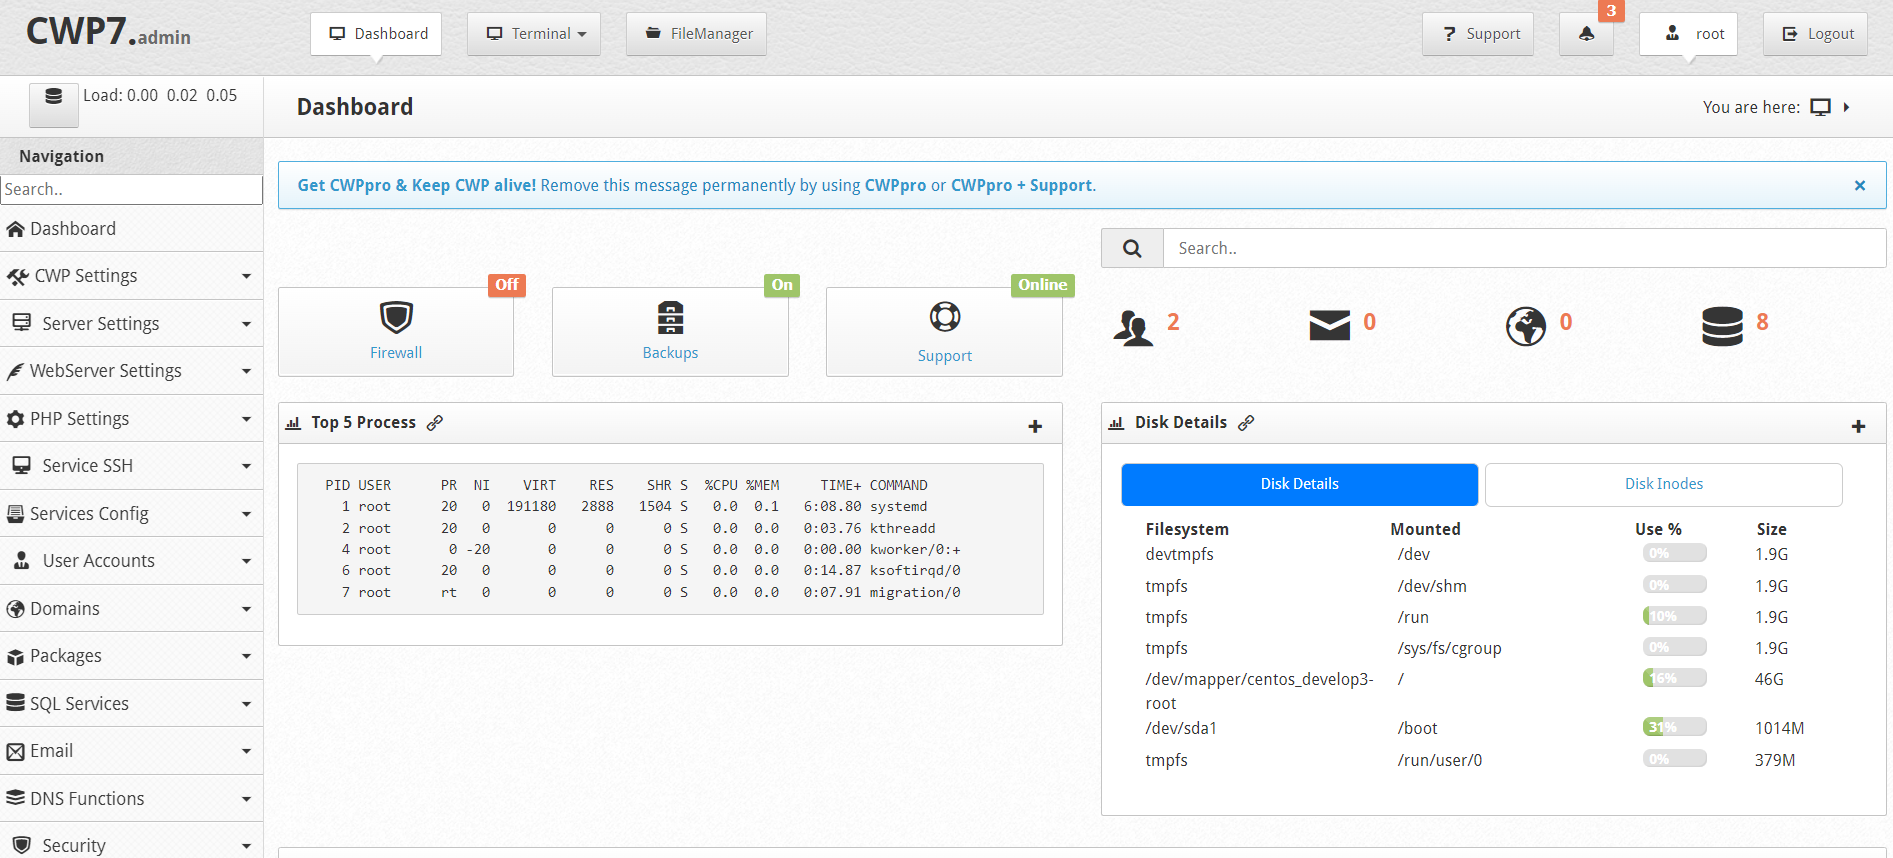
\includegraphics[height=0.3\textheight]{CWP_server.png}
    \caption[CWP van CentOs development server]{CWP van CentOs development server}
    \label{fig:centos_server}
\end{figure}
\subsection{\IfLanguageName{dutch}{Server}{Server}}
De tests worden uitgevoerd op een server die wordt gehost door Sinergio. De server draait op Linux distributie CentOS 7, waarbij bepaalde 
beveiligingsfunctionaliteiten tijdelijk zijn uitgeschakeld om de tests correct te kunnen uitvoeren op de applicaties. Zo is er op de server 
geen firewall geactiveerd en is ModSecurity ook uitgeschakeld zoals je kan zien op de figuur \ref{fig:centos_server}. Dit is 
zo ingesteld om te voorkomen dat het IP-adres van de tester zou worden geblokkeerd tijdens het simuleren van een brute 
force-aanval op een hoger niveau dan de applicatie zelf.

ModSecurity is een open-source webapplicatie firewall (WAF) die bescherming biedt tegen verschillende soorten aanvallen door 
verdachte HTTP-verzoeken te filteren en blokkeren. Het wordt vaak gebruikt om applicaties te beschermen tegen bedreigingen 
zoals SQL-injecties, XSS-aanvallen en brute force-aanvallen. Door ModSecurity tijdelijk uit te schakelen, kunnen de testen 
worden uitgevoerd zonder dat de ingebouwde beveiligingsmaatregelen op serverniveau onbedoeld interfereren met de testresultaten.

Bovenop de CentOs 7 server is een Control Web Panel (CWP) geïnstalleerd. Dit is een webhosting controlepaneel dat
een grafische interface biedt voor het beheren van webhosting servers. CWP biedt een breed scala aan functies zoals
servermonitoring, bestandsbeheer en e-mailbeheer, waardoor het een handige tool is voor het beheren van webhostingomgevingen.

De CentOs server wordt bij Sinergio gebruikt als development- of test server, waardoor het kan worden gehanteerd voor het 
testen van webapplicaties voor ze naar productie worden overgeplaatst. De productie servers daarentegen worden ondersteund 
door Linux 8.

\subsection{\IfLanguageName{dutch}{Wordpress}{Wordpress}}
WordPress is een veelzijdig contentmanagementsysteem (CMS) dat wereldwijd wordt gebruikt door miljoenen websites, variërend van 
eenvoudige blogs tot uitgebreide e-commerceplatforms. De aantrekkingskracht van WordPress ligt in de gebruiksvriendelijke 
interface en de enorme flexibiliteit die het biedt. Gebruikers kunnen kiezen uit duizenden thema's en plugins om hun site 
naar wens aan te passen, zonder dat er verregaande programmeerkennis nodig is. 

Bovendien is WordPress open-source, wat inhoudt dat de 
gemeenschap voortdurend bijdraagt aan de verbetering en veiligheid van het platform. Dankzij de combinatie van gebruiksgemak, 
aanpasbaarheid en de brede ondersteuning door de gemeenschap blijft WordPress de voorkeur genieten van zowel beginnende als 
ervaren webontwikkelaars.

Een belangrijke aanvulling op WordPress is de Wordfence-plugin, een populaire beveiligingstool die specifiek is ontworpen 
voor WordPress-websites. Wordfence biedt uitgebreide bescherming tegen malware, brute force-aanvallen en andere online 
bedreigingen die websites kunnen treffen. Met functies zoals firewallregels, malware-scanning en inlogbeveiliging helpt 
Wordfence gebruikers om hun sites veilig en betrouwbaar te houden. Door de integratie van deze beveiligingslagen kunnen 
website-eigenaars zich richten op het creëren van content en het beheren van hun online aanwezigheid, terwijl ze gerust 
kunnen zijn over de beveiliging van hun website.

In het verdere verloop van deze studie worden de testen zowel uitgevoerd op een wordpress omgeving met als zonder 
beveiligingsplugin.

\subsection{\IfLanguageName{dutch}{Laravel}{Laravel}}
Laravel is een krachtig en veelzijdig PHP-framework dat populair is onder ontwikkelaars voor het bouwen van robuuste 
webapplicaties. Het staat bekend om zijn elegantie en eenvoud, zoals beschreven wordt in \nameref{sec:Webomgevingen} 
uit de literatuurstudie, waardoor het zowel beginners als ervaren ontwikkelaars aanspreekt. 

Laravel biedt een rijke set aan tools en bibliotheken die het ontwikkelen van complexe toepassingen eenvoudiger 
maken, zoals ingebouwde authenticatie, routing en een intuïtief templating-systeem. Het framework volgt de MVC-architectuur 
(Model-View-Controller), wat zorgt voor een gestructureerde en onderhoudbare codebase. Bovendien stimuleert Laravel het 
gebruik van best practices in webontwikkeling, zoals beveiligde codering en testen. Hierdoor vormt het een betrouwbare keuze 
voor het bouwen van veilige en schaalbare applicaties. 

Dankzij de uitgebreide documentatie en een actieve gemeenschap, kunnen 
ontwikkelaars snel aan de slag en blijven ze ondersteund tijdens het ontwikkelproces.

\begin{figure}
    \centering
    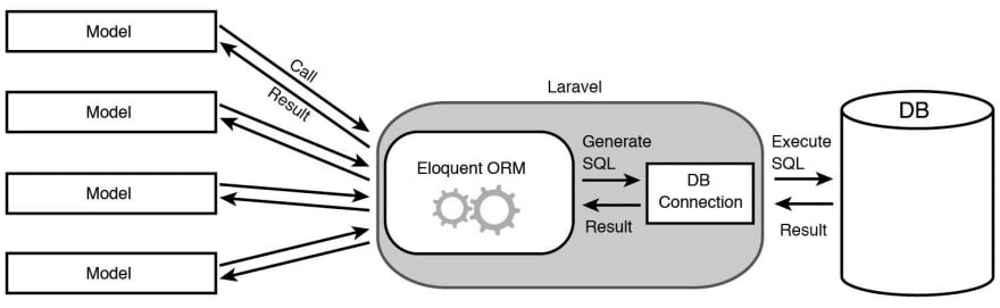
\includegraphics[height=0.2\textheight]{laravel_schema.png}
    \caption[Laravel ORM schema]{Laravel ORM schema ~\autocite{2020}}
    \label{fig:laravel_schema}
\end{figure}

Ook het ORM (Object Relational Mapping) systeem van Laravel is een belangrijke troef. Dit systeem maakt het mogelijk om 
het systeem te beschermen van SQL-injectie via de Eloquent ORM. Dit gebeurt door middel van PDO (PHP Database Objects) binding, waarbij de
gebruiker geen directe SQL queries kan uitvoeren. Eloquent slaat de SQL commando's eerst op en zet de onveilige code om 
naar tekst. Het schema van Laravel is te zien op deze foto \ref{fig:laravel_schema}.
